In order to interact with the robot aside of speech, a web-based \gls{gui} has been designed.
The interface has been made with HTML5\footnote{\texttt{https://github.com/tue-robotics/tue\_mobile\_ui}} and is hosted on the robot itself.
This allows multiple users on different platforms (\eg\ Android, iOS) to access functionality of the robot. The interface is implemented in JavaScript with AngularJS and it offers a graphical interface to the Robot API\footnote{\texttt{https://github.com/tue-robotics/robot-api}} which exposes all the functionality of the robot.
Figure~\ref{fig:webgui_architecture} gives an overview of the connections between these components.

\begin{figure}[H]
	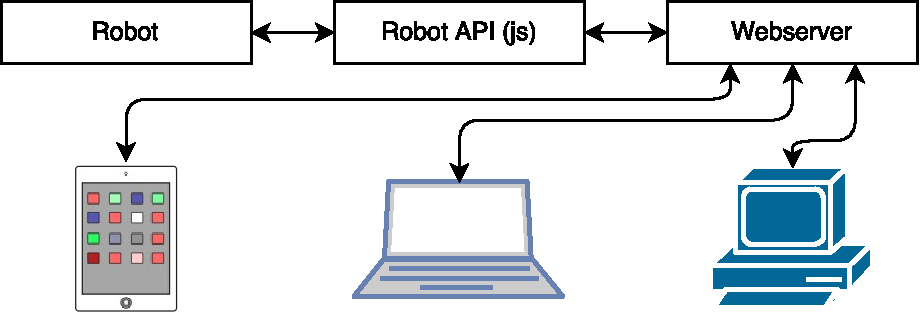
\includegraphics[width=\linewidth]{webgui_architecture}
	\caption{
		Overview of the WebGUI architecture.
		The robot's functionalities are exposed with the Robot API that is implemented in JavaScript.
		The webserver that is hosting the \protect\gls{gui} connects this Robot API to a graphical user interface that is offered to multiple clients on different platforms.}
	\label{fig:webgui_architecture}
\end{figure}
